%\section{Raisonnement(s)}



\begin{frame}
	\titre{Introduction}
	
	\begin{description}[labelindent=6pt,style=multiline,leftmargin=1.3in]
		 \setlength\itemsep{1em}
		 \item[Raisonnement] Application d'une procédure \pause (ou d'un algorithme) \pause qui, à partir d'un ensemble de propositions considérées comme vraies (les \textbf{prémisses}), aboutit à une proposition (\textbf{conclusion})\pause
		 \item[Remarques] Une définition parmi d'autres\pause
		 \item[] Mécanisme cognitif et naturel \pause qu'on essaye de représenter avec des théories / outils linguistiques et mathématiques\pause
		 \item[] Rien dans la définition n'impose la validité (de la procèdure ou de son application)
 	\end{description}
\end{frame}



\begin{frame}
	\titre{Introduction}
	On fera donc la distinction entre raisonnements \textbf{rigoureux} et \textbf{non-rigoureux} \pause \newline
	
	Un raisonnement est \textbf{rigoureux} s'il est \textbf{valide} \pause (waouh) \pause\newline

On qualifiera de \textbf{non-rigoureux} des raisonnements qui ne sont pas valides\pause, mais qui sont utilisés en pratique, leur absence de validité théorique étant compensée par une bonne applicabilité \pause (ils peuvent être faux, mais marchent souvent bien)\pause \newline

Les raisonnements non-rigoureux ont une régularité qui permet de les formaliser \pause (contrairement aux sophismes par exemple)\pause \newline

Cf la distinction \textbf{algorithme} / \textbf{heuristique}
		 \end{frame}




\begin{frame}
	\titre{Raisonnements rigoureux}
	
	\begin{description}[labelindent=6pt,style=multiline,leftmargin=1.3in]
		 \setlength\itemsep{1em}
		 \item[En gros] Combinaison des prémisses via des \textbf{lois logiques} \pause et \textbf{rien d'autre}\pause
		 \item[Remarque] Ca ressemble à Port-Royal \pause en encore plus raide ! (cf le syllogisme 6 du dernier cours)\pause
		 \item[] Ce type de raisonnement intéresse principalement les matheux \& cie (cf le \textit{model-checking})
		  	\end{description}
\end{frame}

\begin{frame}
	\titre{Ex : calcul propositionnel}
	
	\begin{description}[labelindent=6pt,style=multiline,leftmargin=1.3in]
		 \setlength\itemsep{1em}
		 \item[En gros] Plein de `petites règles`, généralement intuitives\pause
		 \item[Exemples] De `P et Q`, on peut déduire P \pause(ou Q)\pause
		 \item[] De `P`, on a `P ou Q` \pause (`ou` inclusif !)\pause
		 \item[] De `non (non P)` on déduit `P`\pause
		 \item[] etc ...
  	\end{description}
\end{frame}


\begin{frame}
	\titre{Ex : calcul propositionnel}
	
Plus compliqué : le `Si P, alors Q`\pause \newline
	
Rappel du DM2 : vous avez promis à votre amie Chloé d'aller la voir demain s'il fait beau. On suppose d'abord que vous êtes du genre à tenir votre promesse\pause \newline

Vous vous levez et il fait beau, donc vous \pause allez voir Chloé\pause \newline

Vous vous levez et il fait moche, donc vous \pause faites autre chose \pause ou pas ! \pause Prise \textbf{littéralement} (cf la discussion sémantique / pragmatique), votre promesse ne vous empêche, dans aucun cas, d'aller voir Chloé (et puis c'est toujours sympa une surprise).
\end{frame}

\begin{frame}
	\titre{Version abstraite : `Si P, alors Q`}
	
On est (normalement) d'accord qu'on a `non-P ou P`\pause \newline

La proposition `Si P, alors Q` impose que, dans toute situation où P est vraie, Q l'est également. \pause On \textit{enrichit} donc `non-P ou P`, qui devient `non-P ou (P et Q)`\pause \newline 
	
Ca traduit bien `Si P, alors Q`, mais on peut faire mieux \pause : si P est fausse, la partie droite (`P et Q`) est fausse aussi, mais c'est \textit{rattrapé} par la partie gauche (car non-P est alors vraie)\pause  \newline
 	
A l'inverse, si P est vraie, la prop. devient simplement `Q`\pause \newline
 	
On n'a donc pas besoin du `P` à droite, `Si P, alors Q` se réécrit donc en \textbf{`non-P ou Q`}
\end{frame}


\begin{frame}
	\titre{Ex : calcul propositionnel}
	
Plus compliqué : le `Si P, alors Q`\newline
	
Rappel du DM2 : vous avez promis à votre amie Chloé d'aller la voir demain s'il fait beau. \pause On suppose maintenant que vous ne vivez que pour trahir vos promesses\pause \newline

Vous vous levez et il fait beau, donc vous \pause n'allez surtout pas voir Chloé\pause \newline

Vous vous levez et il fait moche, donc vous \pause êtes foutu(e) ! \pause Votre promesse ne vous forçait à rien en cas d'absence de beau temps, il n'y a donc pas d'interdit à enfreindre. \pause\newline 

(ça vous apprendra à être méchant(e))

\end{frame}



\begin{frame}
	\titre{non-(Si P, alors Q) }
	
La seule façon de rompre la promesse `Si P, alors Q`, c'est d'être en situation où `P` est vraie et ne surtout pas faire `Q`\newline \pause

La contradiction de `Si P, alors Q` est donc \pause \textbf{`P et non-Q`} \newline \pause

Notation : `non-P`, c'est la proposition contradictoire (pour les linguistes), ou la négation (pour les logiciens) de P \pause \newline

Rappel : `non-(P ou Q)` $\equiv$ `(non-P et non-Q)`\newline
\textcolor{white}{Rappel :} `non-(P et Q)` $\equiv$ `(non-P ou non-Q)` \newline \pause

Si on cherche la proposition contradictoire de `P et non-Q`, on a `non-P et non-non-Q`\pause, c'est à dire `non-P ou Q` \pause (magie !)

\end{frame}



\begin{frame}
	\titre{Ex : raisonnement par l'absurde }

Rappel : toute propriété est soit vraie, soit fausse (`P ou non-P`). \pause Si on montre que la négation non-P est fausse, alors P est automatiquement vraie\pause\newline

Pour montrer qu'une proposition est fausse, on montre qu'en l'introduisant dans les hypothèses, on \textbf{crée} un paradoxe \pause (qui ne serait pas là sinon !)\pause\newline 
	
Exemple dans le DM2 : \pause voir le DM2 (de rien)

\end{frame}


\begin{frame}
	\titre{Ex : induction complète}
	
		\begin{description}[labelindent=6pt,style=multiline,leftmargin=1.3in]
		 \setlength\itemsep{1em}
		 \item[En gros] Montrer que tous les éléments d'un ensemble partagent une propriété\pause
		 \item[Exemple bourrin] \begin{tabular}[t]{l}
Diane est cool\\
Elsa est cool\\
Jules est cool\\
Mes seuls amis sont Diane, Elsa et Jules\\
\hline
Tous mes amis sont cool
\end{tabular}\pause
		 \item[Remarque] L'ensemble est fini, donc on peut faire la preuve par énumération. \pause C'est pas hyper intéressant
  	\end{description}

\end{frame}

\begin{frame}
	\titre{Ex : induction complète}
	Une récurrence (arithmétique) nous permet de prouver une propriété pour un ensemble infini d'éléments\pause \newline
	
		\begin{description}[labelindent=6pt,style=multiline,leftmargin=1.3in]
		 \setlength\itemsep{1em}
		 \item[Exemple] Tout entier naturel est soit pair, soit impair\pause
		 \item[Initialisation] C'est vrai pour $0$ ($0 = 2 \times 0$)\pause
		 \item[Hérédité] Soit n qui est soit pair, soit impair\pause  	\end{description}
	
		 Si $n$ pair, $n = 2 \times p$, donc $n = 2 \times p + 1$, donc $n+1$ impair\pause\newline
		 
Si $n$ impair, $n = 2 \times p + 1$, donc $n = 2 \times (p + 1)$, $n+1$ pair\pause\newline

		 Conclusion, 0 a la propriété voulue, et elle se \textit{transmet} d'entier en entier. \pause C'est un cas particulier d'induction (structurelle)


\end{frame}




\begin{frame}
	\titre{L'induction non-rigoureuse}
	
		\begin{description}[labelindent=6pt,style=multiline,leftmargin=1.3in]
		 \setlength\itemsep{1em}
		 \item[En gros] Une induction incomplète, cad qui généralise à partir d'un sous-ensemble \pause
		 \item[Remarque] Même si \textit{les données} sont représentatives, le raisonnement n'est pas \textbf{valide}\pause
		 \item[Exemple]
		  \begin{tabular}[t]{l}
Alien est bien\\
Alien 2 est (trop trop) bien\\
Alien 3 est bien\\
\hline
Tous les films Alien sont biens\\
\end{tabular}\pause
		 \item[Exemple bis] La dinde inductiviste de Russel\pause
  	\end{description}
  	En pratique, on est obligés de faire des inductions non rigoureuses (ou généralisations), ce qui est une science en soi
\end{frame}

\begin{frame}
	\titre{L'analogie}
	
		\begin{description}[labelindent=6pt,style=multiline,leftmargin=1.3in]
		 \setlength\itemsep{1em}
		 \item[En gros] Un objet A a une propriété B\pause
		 \item[] On remarque des correspondances entre A et un autre objet C\pause
		 \item[] On essaie de retrouver dans C une propriété D correspondant à B\pause
		 \item[Exemple] ?
  	\end{description}
\end{frame}


\begin{frame}
	\titre{L'abduction}
	
		\begin{description}[labelindent=6pt,style=multiline,leftmargin=1.3in]
		 \setlength\itemsep{1em}
		 \item[ou] \textit{Inférence de la meilleure explication}\pause
		 \item[En gros] On observe la \textbf{conclusion} d'un raisonnement familier ou naturel ou très probable, dont éventuellement certaines prémisses sont en place\pause
		 \item[] Et on infère que la ou les prémisses manquantes doivent également être vraies\pause
		 \item[Exemples] La route est mouillée\pause, donc il a plu\pause
		 \item[] Il y a des miettes de pain dans votre cuisine le matin\pause, votre colloc a dû se préparer un encas pendant la nuit
  	\end{description}
\end{frame}



\begin{frame}
	\titre{Ex : le colonel Moutarde}

La démonstration donnée est une preuve logique de la culpabilité de Mr Flap \pause mais ne dit pas comment le meurtre a eu lieu ou pourquoi\pause\newline

A l'inverse, d'autres indices (non-utilisés dans la preuve) donnent un déroulé \textbf{possible} (sans doute même le plus \textbf{probable}) du meurtre\pause, \textbf{mais ça ne prouve pas la culpabilité de Mr Flap}\newline\pause
	
Rappel : en logique, on exige rien de moins que le béton armé\pause\newline 

Ca ne veut pas dire que cette approche n'a aucun intérêt, mais ça relève alors des probas (cf le maximum de vraisemblance)
\end{frame}



\begin{frame}
	\titre{DM3 : raisonnement 1}

Le fait que l'élève n'ait pas eu une bonne note parce qu'il / elle n'a pas travaillé n'est pas la seule explication, mais c'en est une \textit{naturelle}, une des plus probables. \pause Le prof fait donc une \textbf{abduction}\pause\newline

C'est un raisonnement qui n'est, par essence, pas rigoureux, et on peut en effet imaginer de nombreuses raisons pour lesquelles l'élève aurait échoué (et vous avez bien plus d'imagination que moi à ce niveau)\pause\newline

Ce qu'il manque au prof, c'est le fait qu'avoir travaillé \underline{garantit} la bonne note, auquel cas le raisonnement serait valide \pause (ou une surveillance 24/7 de l'élève si j'en crois vos copies)
\end{frame}

\begin{frame}
	\titre{DM3 : raisonnement 2}

Le raisonnement du politique est que la stratégie économique marche pour l'Allemagne, et que la France et l'Allemagne sont deux pays similaires, donc que le résultat peut se \textit{transférer} à la France. \pause C'est une \textbf{analogie}, qui est un raisonnement par nature non-rigoureux\pause\newline

Certains ont fait la remarque que le raisonnement n'est pas si non-rigoureux que ça, puisque le politique dit que la France \textbf{pourrait} s'inspirer du modèle économique pour aller mieux. \pause Pour moi, ambiguïté entre `La France a plusieurs options \textit{sûres}, dont s'inspirer de l'Allemagne` (non-rigoureux) et `Ptet que l'Allemagne ça marchera` (non-non-rigoureux, parce que quasiment vide de sens)

\end{frame}

\begin{frame}
	\titre{DM3 : raisonnement 2 - bonus}

L'analogie dit seulement que ce qui marchera pour l'Allemagne marchera aussi pour la France, mais pas que c'est la seule solution\pause\newline

Quand le politicien dit que pour améliorer sa situation, la France \textbf{\underline{doit}} s'inspirer du modèle Allemand, il sort donc de ce cadre (et il dit encore plus n'importe quoi (au niveau du raisonnement))

\end{frame}

\begin{frame}
	\titre{DM3 : raisonnement 3}

Si vous déduisez que Chloé est allée voir \textit{Millennium Actress}\footnote{Elle aurait d'ailleurs fort raison, c'est un film magnifique}, c'est non-rigoureux. \pause De par les conditions de l'énoncé, c'est l'explication la plus probable (\textbf{abduction}), mais elle aurait tout aussi pu regarder un autre film chez elle\pause\newline

D'ailleurs, en supposant que Chloé dit la vérité et qu'aucun imprévu n'est arrivé, la seule chose qu'on peut déduire de son absence est qu'elle a regardé un film :\pause\newline

$P = $ Chloé vient / est venue ;  $Q = $ Chloé a regardé un film\newline\pause

On a $((\neg P \rightarrow Q) \wedge \neg P)$, d'où on peut déduire $Q$ (règle \textbf{modus ponens} du \textbf{calcul propositionnel})

\end{frame}


\begin{frame}
	\titre{DM3 : raisonnement 3}

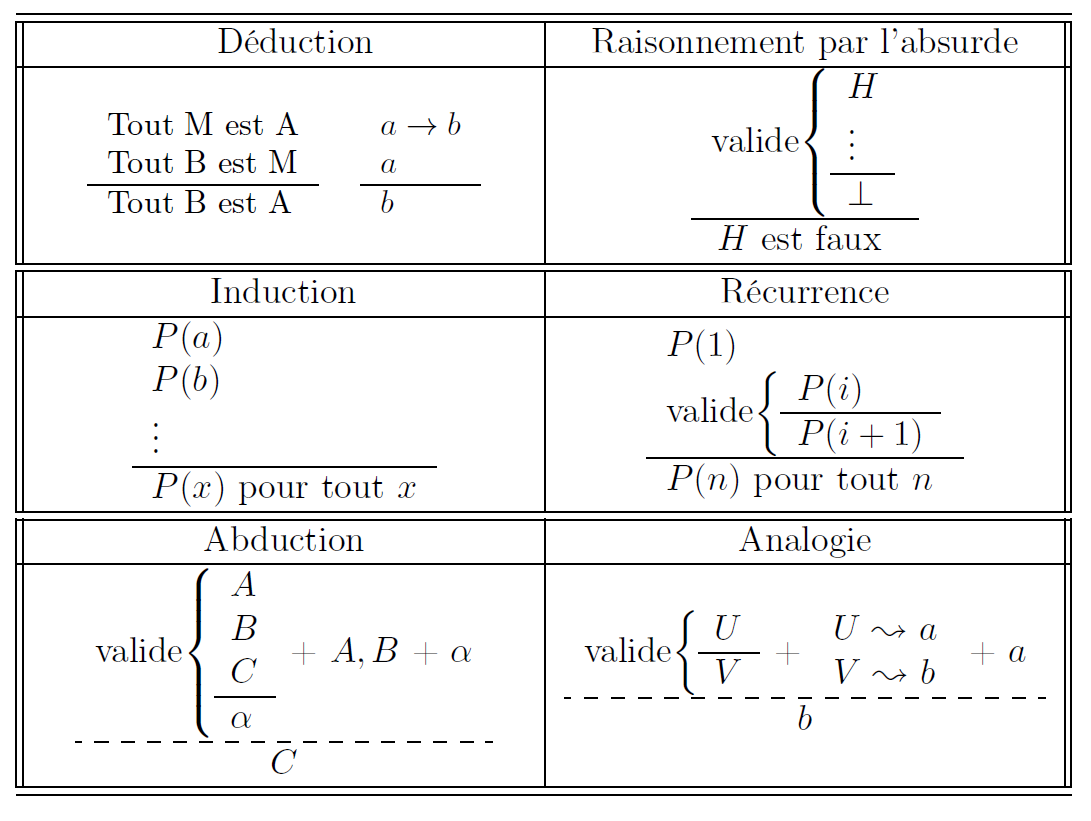
\includegraphics[scale=0.32]{raisonnements.png}

\end{frame}
